
\chapter{Framework Architecture}
\label{ch:architecture}
\section{Used Technologies}
\label{sec:technologies}

\subsection{3D FPS Game Engine}


VIZIA Environment was build around FPS (First Person Shooter) game Doom and it's game engine's modernized version -- ZDoom. It is shown in Figure~\ref{fig:doom}.  
\begin{figure}
\centering
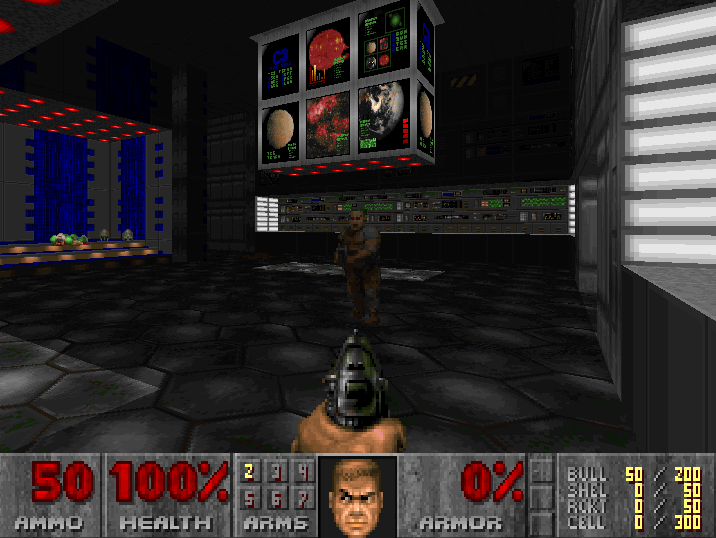
\includegraphics[scale=0.6]{doom.png}
\caption{Screenshot of Doom}
\label{fig:doom}
\end{figure}
Doom was selected from 6 other recognizable FPS games:
\begin{itemize}
\item Quake III Arena 
\item Doom 3
\item Half-Life 2 
\item Unreal Tournament 2004
\item Unreal Tournament
\item Cube
\end{itemize}
Comparision between mentioned games is shown in Table~\ref{tab:engines}.
Some of the criteria had to be subjective (System requirements, Code complexity), becouse they were based on analysis of engine's code in the context of internal architecture, easiness of modification and performance. 
  

\begin{table}[]
\centering
\caption{Overview of 3D FPS games considered as base of VIZIA environment}
\label{tab:engines}
\begin{tabular}{|p{2cm}||p{1.3cm}|p{1.3cm}|p{1.3cm}|p{1.3cm}|p{1.3cm}|p{1.3cm}|p{1.3cm}|}
\hline
Game                      & Quake III: Arena \cite{quake1}~\cite{quake2} & Doom \cite{doomreq}~\cite{zdoom}~\cite{zdoom-wiki}  & Doom 3 \cite{d3req}~\cite{idtech4}    & Half-Life 2 \cite{half2}~\cite{source} & Unreal Tournament 2004 \cite{ut04rqe}~\cite{ue2} & Unreal Tournament \cite{ue4req}~\cite{ue4faq} & Cube~\cite{cube}        \\ \hline
Game Engine               & ioquake3         & zdoom & id tech 4 & Source      & Unreal Engine 2        & Unreal Engine 4   & Cube Engine \\ \hline
Relase year               & 1999             & 1993  & 2003      & 2004        & 2004                   & --\footnotemark              & 2001        \\ \hline
Open Source               & \OK              & \OK   & \OK       &             &                        & \OK               & \OK         \\ \hline
Licence                   & GPLv2            & GPL   & GPLv3     & Closed      & Closed                 & Custom            & ZLIB        \\ \hline
Language                  & C                & C++   & C++       & C++         & C++                    & C++               & C++         \\ \hline
DirectX                   &                  &       &           & \OK         &                        & \OK               &             \\ \hline
OpenGL                    & \OK              & \OK\footnotemark   & \OK       & \OK         & \OK                    & \OK               & \OK         \\ \hline
Software Render           &                  & \OK   &           &             &                        &                   &             \\ \hline
Windows                   & \OK              & \OK   & \OK       & \OK         & \OK                    & \OK               & \OK         \\ \hline
Linux                     & \OK              & \OK   &           & \OK         & \OK                    & \OK               & \OK         \\ \hline
Mac OS                    & \OK              & \OK   & \OK       & \OK         & \OK                    & \OK               &             \\ \hline
Scripting                 &                  & \OK   &           & \OK         & \OK                    & \OK               & \OK         \\ \hline
Custom assets             & \OK              & \OK   & \OK       & \OK         & \OK                    & \OK               & \OK         \\ \hline
Map editor                & \OK              & \OK   & \OK       & \OK         & \OK                    & \OK               & \OK         \\ \hline
Multiplayer               & \OK              & \OK   &           &             & \OK                    & \OK               & \OK         \\ \hline
Engine access             & Code             & Code  & Code      & SDK         & SDK                    & SDK               & Code        \\ \hline
Small resolutions         & \OK              & \OK   & \OK       & \OK         & \OK                    & \OK               & \OK         \\ \hline
Screen buffor access      & \OK              & \OK   & \OK       &             &                        & \OK               & \OK         \\ \hline
System requirements       & Low              & Low   & Medium    & Medium      & Medium                 & High              & Low         \\ \hline
Disk space                & 70MB             & 40MB  & 2GB       & 4,5GB       & 6GB                    & \textgreater10GB\footnotemark  & 35MB        \\ \hline
Code complexity           & Medium           & Medium& High      & NA          & NA                     & High              & Low         \\ \hline
Brand recognition         & 41,1             & 99    & 99        & 36,6        & 1,2                    & 1,2               & 0,1         \\ \hline
Active community          & \OK              & \OK   & \OK       & \OK         &                        & \OK               &             \\ \hline
Free original assets      &                  &       &           &             &                        & \OK               & \OK         \\ \hline
\end{tabular}
\end{table}
\addtocounter{footnote}{-2}
\footnotetext{Unreal Tournament is in pre-alpha phase; relase date is unknown.}
\stepcounter{footnote}
\footnotetext{GZDoom, ZDoom fork, is OpenGL based.}
\stepcounter{footnote}
\footnotetext{Disk requirements are yet unknown, but they will be greater than requirements of Unreal Engine 4.}


Lack of scripting support and unaccessible screen buffer were considered as a critical factors for rejecting such game and accessing engine's logic only by SDK was considered as a major drawback, so Unreal Tournament 2004 and Half-Life 2 could not be accepted.
Multi-threaded or client-server architecture would make it difficult to fully control speed of the execution, therefore Quake III Arena had to be rejected.
Doom 3 had to be ignored not only for this reason, but also becouse of its complexity, Windows-only tools and OS-dependent rendering mechanisms.
Cube's lack of recognizability was reason of rejecting it, although it comes with highly intuitive map editor.
Despite active community and great capabilities Unreal Tournament was out of question, becouse of its very high system requirements.


ZDoom based Doom met most of given requirements and allowed to implement features that would by hard or impossible to achieve in other games eg. offscreen rendering and reward computation.
Although Doom wasn't greatly used in research on reinforcement learning, it's recognizability exceeds Unreal Tournament brand.
Originally Doom was designed to work in 320x240 resolution and even so modern implementation allow bigger resolutions, it still utilizes same low resolution textures and rendering algorithm what makes it perfect for generating small visual input data (320x240 or smaller) for reinforcement learning algorithm.
Code analysis showed that access to game logic should be easy, as it is not object-oriented code.
Unique Doom's feature is software renderer. Because of that it could be used without desktop environment (eg. remotely over ssh).
Doom's gameplay is quite simple compared to newer FPS games as it consists mostly of running around and shooting and possible actions could be easly translated for reinforcement learning needs. 






\subsection{Operating System}


Linux has been choosen as a target operating system for this environment.
Compilation tool-chain based on CMake and makefile allowed to automate building process and simplify project configuration.



\subsection{Game Controller and API}


The basic module for control over Doom - game controller - was written in C++ with usage of Boost library.
It allowed to use Boost::interprocess library in both ZDoom and game controller, as ZDoom was written in C++, what made connecting game controller and game easier than it would be using low level language on the engine side and high level language for the controller.
Experimental Boost::process library was used for control over Doom process.


Above the controller the higher layer of abstraction was implemented defining Application Programming Interface for intelligent agents modules.
It was also developed in C++ what allowed to provide bindings to Python and Java, with possibility to add another languages eg. Lua, Julia.


Python API was considered as main way of controlling VIZIA Environment by users.
Bindings were prepared by using Boost::python library.
This language is one of the most popular in data science~\cite{ds_lang} and wide known as it is taught at many universities all around the world~\cite{pythons_schools}.
There are many machine learning libraries for Python such as scikit-learn or PyBrain.
Because of that providing fully functional Python API was one of the biggest priorities of this project.


For Java bindings Java Native Interface (JNI) was used.


\subsection{Map Editor and Scripting}


Creation of test environments has been made possible by using tools developed by Doom's community for maps and scripts editing: SLADE 3 and Doom Bulider 2. Those tools utilizes ACC -- compilter for Action Code Script (ACS), language, which is supported in ZDoom engine.
This topic was discussed further in Chapter~\ref{ch:scenarios}.

\section{Architecture}\label{sec:architecture}
	\begin{figure}
			\centering
			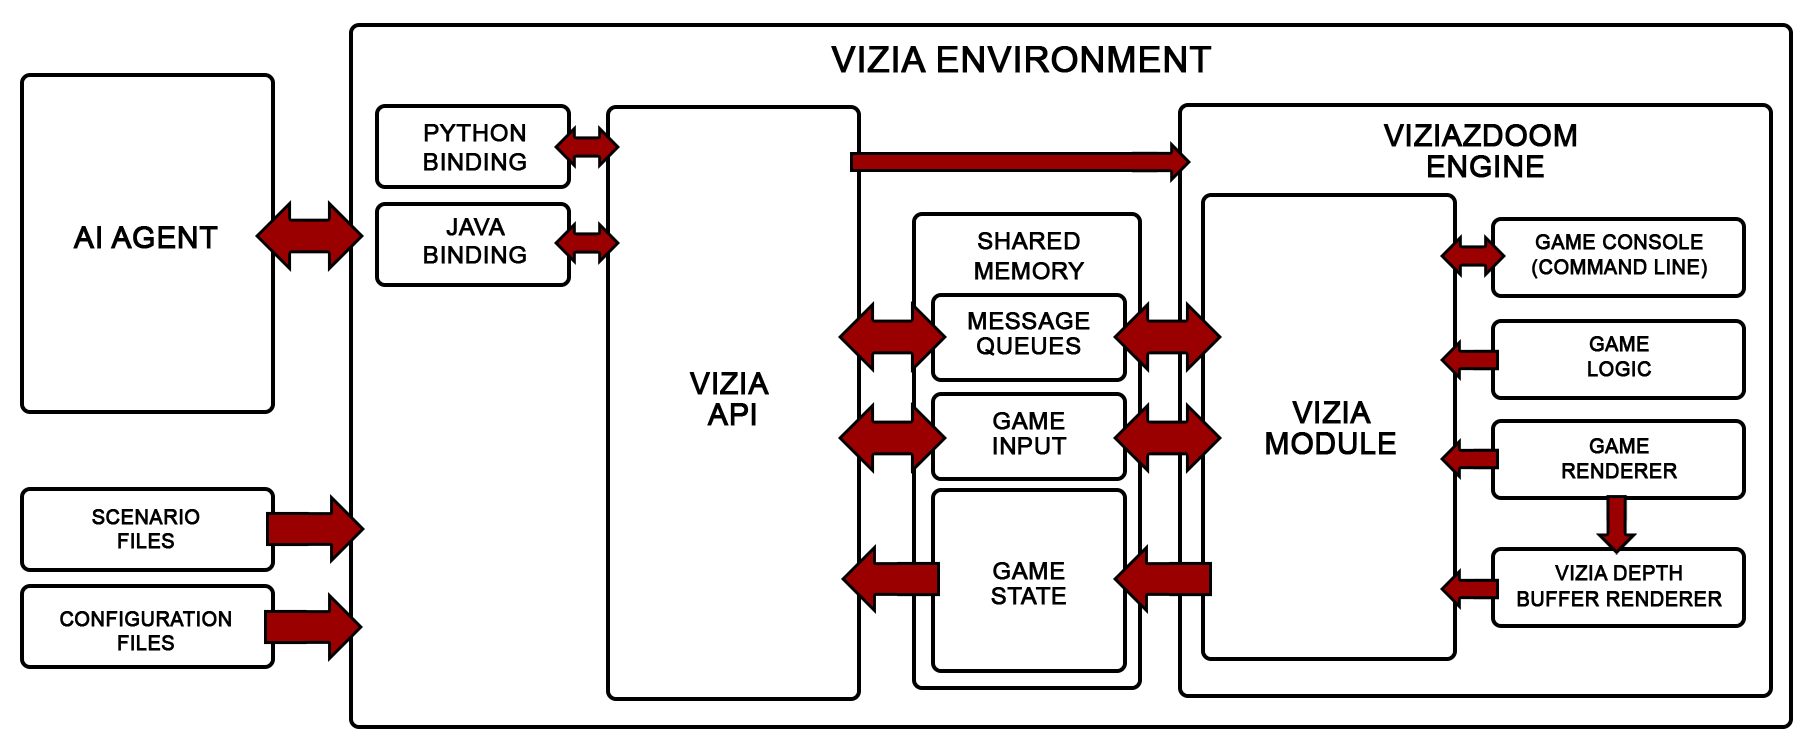
\includegraphics[scale=0.25]{architecture_diagram.png}
			\caption{Architecture of Vizia Environment.}\label{fig:architecture_diagram}
	\end{figure}

The main components of Vizia environament:
    \begin{itemize}
    \item Vizia library -- which provides a DoomGame API that allows user to configure, launch and play the game in several flow control modes.
    \item ViziaZDoom -- modified ZDoom engine with a Vizia module to communicate with a DoomGame object, control the game flow and adding additional rendering modes. It can act as a process under the control of the DoomGame object, Dome engine used for testing in Doom editors or as standalone process.
    \item Python and Java bindings -- allowing the use of the DoomGame API in these languages.
    \end{itemize}


\subsection{The separate API and game processes}\label{sec:architecture_separate_processes}

When the API user initiates the processing, the DoomGame object creates a second thread that starts ViziaZDoom process with the appropriate settings and supervises it. From this point the API and the game communicate using only a shared memory.


\subsection{Shared memory to communicate}\label{sec:architecture_shared_memory}

During initialization set of spaces are created in the shared memory space, which includes:
    \begin{itemize}
    \item A pair of message queues to control the processing flow and sending commands to the game.
    \item A shared memory area to exchange information about game input status. Both the API process and the game process reads and writes to shared memory.
    \item Shared memory areas where the game provides state of the game. These are the values of the variables games necessary to control the processing variables and a copy provided to you buffor wyrenderowanego in the game image. The game process saves to the memory, the process of API support.
    \end{itemize}
All shared memory spaces have unique names for each DoomGame object, which allows the coexistence of multiple instances.


\subsection{Vizia module inside ViziaZDoom}\label{sec:architecture_inside_viziazdoom}

Vizia module inside the engine initializes the shared memory to exchange information with this instance of the game. Then controls the flow of the game depending on the processing mode, and received messages and determines the following processing steps:

    \begin{itemize}
    \item Starting processing of the next game tic.
    \item Transmiting commands from the message queue to the game console.
    \item Sending inputu information from shared memory to the game console.
    \item Processing of events that the game window recieved since the last tic.
    \item Rendering the current frame.
    \item Updating the information about the current game state in the shared memory.
    \end{itemize}

\subsection{Flow control modes}\label{sec:architecture_modes}

The DoomGame API implements four flow control modes:
    
    \begin{itemize}
    \item Synchronous player
    \item Synchronous spectator
    \item Asynchronous player
    \item Asynchronous spectator
    \end{itemize}
    
    \subsubsection{Synchronous player mode}\label{sec:architecture_player_mode}
    
        \begin{figure}
			    \centering
			    
\includegraphics[scale=0.25]{player_mode_diagram.png}
			    \caption{Processing flow in synchronous player mode.}\label{fig:player_mode_diagram}
	    \end{figure}
        
	    Synchronous player mode provides synchronous communication between the process that uses the API and the game process. It allows AI agent to make actions as a player. 
	    
	    In this mode, the API and the game processes communicates every tic and are waiting for each other. The game process waits until the API sends a message requesting processing of the next tic and optional update. The game process, after receiving the message, sends input information (AI agent's action) to the game console, process next game tic, and if update was requested renders the current frame and updates the information about the current game state in the shared memory. After this the game process sends a message about completing request and starts waiting for the message processing of the next tic. The process that uses the API waits for the message about completing request.
	    
	    This mode is designed for the singleplayer, the multiplayer will not work correctly - the game net code is disabled in this mode.

    \subsubsection{Synchronous spectator mode}\label{sec:architecture_spectator_mode}

	    \begin{figure}
			    \centering
			    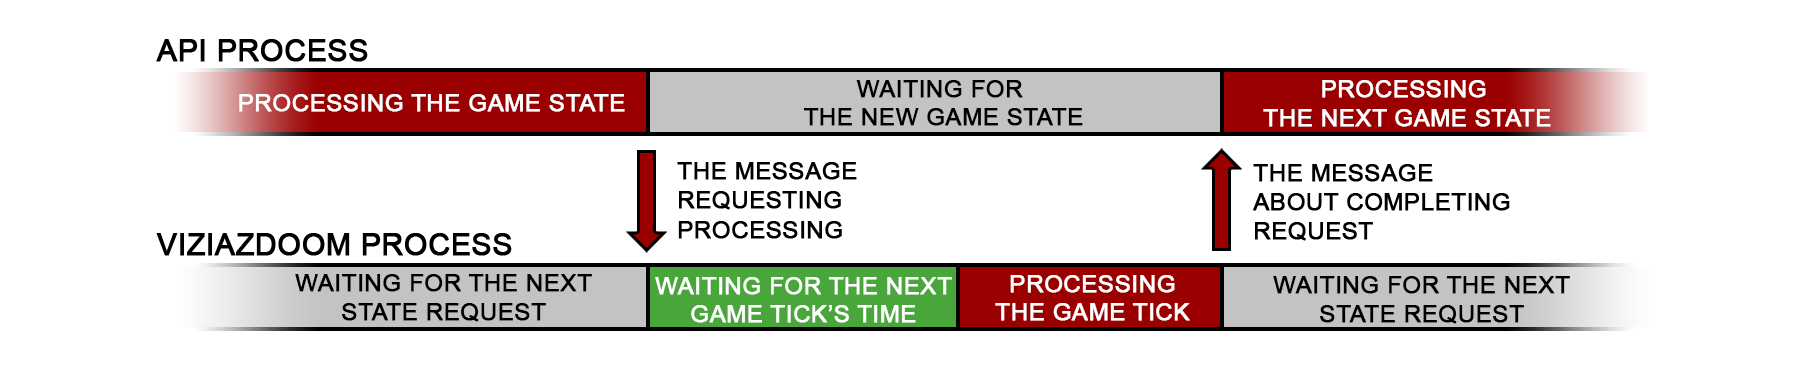
\includegraphics[scale=0.25]{spectator_mode_diagram.png}
			    \caption{Processing flow in synchronous spectator mode.}\label{fig:spectator_mode_diagram}
	    \end{figure}
	    
	    Synchronous spectator mode provides synchronous communication between the process that uses the API and the game process. It allows AI agent to observe a human player's actions. 
	    
	    In this mode the API and the game processes communicates every tic and are waiting for each other. The game process waits until the API sends a message requesting processing of the next tic and optional update. The game process, after receiving the message, process the window input events that have taken place since the last update request (last human player's action), updates the input information in the shared memory, process next game tic and if update was requested renders the current frame and updates the information about the current game state in the shared memory. After this the game process sends a message about completing request and starts waiting for the message processing of the next tic. The process that uses the API waits for the message about completing request.

        Before processing of the next game tic the delay may be introduced in order to ensure the maximum processing speed of 35 tics per second (designed Doom ticrate).
        
        This mode is designed for the singleplayer, the multiplayer will not work correctly - the game network code is disabled in this mode.

    \subsubsection{Asynchronous player mode}\label{sec:architecture_async_player_mode}

	    \begin{figure}
			    \centering
			    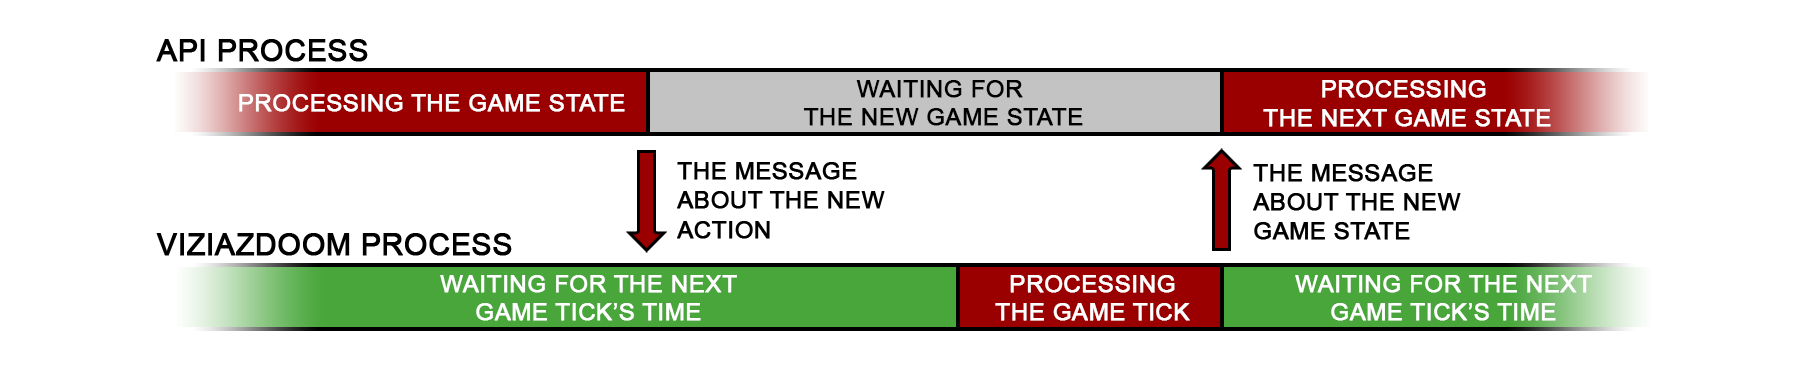
\includegraphics[scale=0.25]{async_player_mode_diagram.png}
			    \caption{Processing flow in asynchronous player mode.}\label{fig:async_player_mode_diagram}
	    \end{figure}
	    
	    Asynchronous player mode provides asynchronous communication between the process that uses the API and the game process. It allows AI agent to make actions as a player. 
	    
	    In this mode, the game process continuously process the game tics a constant speed of 35 tics per second (designed Doom ticrate) without waiting for the API process. The API can send a message requesting update. Before each tic the game process checks if it received a message requesting update. After receiving such the message, it sends the input information (AI agent's action) to the game console, process next game tic, updates the information about the current game state in the shared memory, sends a message about completing request and continues processing of the game tics. The process that uses the API waits for the message about completing request.
	    
	    In this mode, both the singleplayer as well as the multiplayer will work correctly - the game network code is disabled in this mode.

    \subsubsection{Asynchronous spectator mode}\label{sec:architecture_async_spectator_mode}

	    \begin{figure}
			    \centering
			    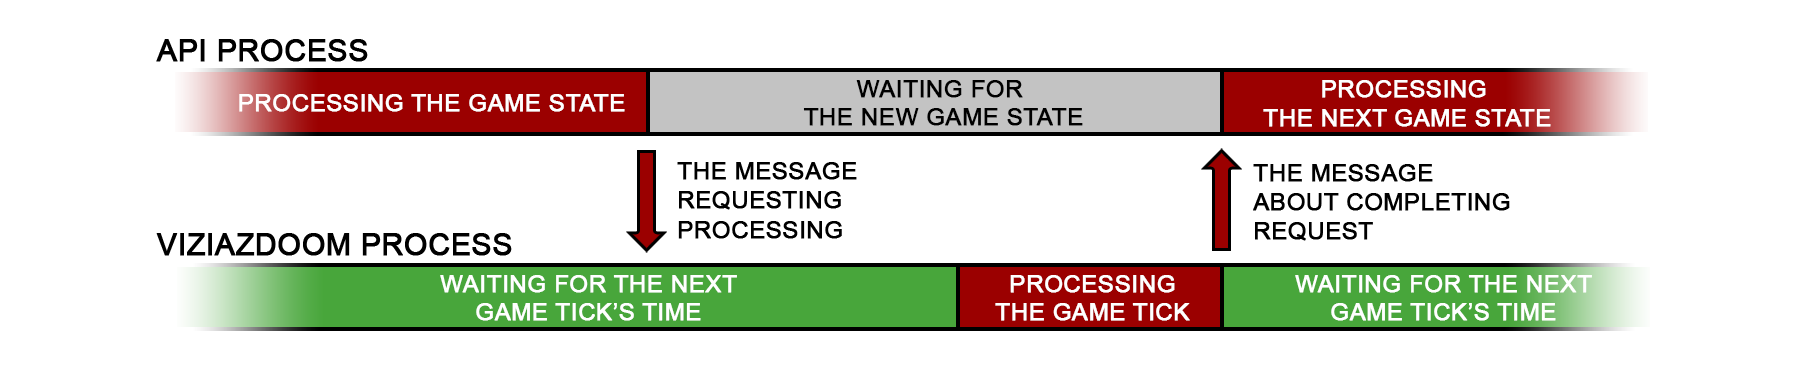
\includegraphics[scale=0.25]{async_spectator_mode_diagram.png}
			    \caption{Processing flow in asynchronous spectator mode.}\label{fig:async_spectator_mode_diagram}
	    \end{figure}
	    
	    Asynchronous spectator mode provides asynchronous communication between the process that uses the API and the game process.It allows AI agent to observe a human player's actions. 
	    
	    In this mode, the game process continuously process the game tics at a constant speed of 35 tics per second (designed Doom ticrate) without waiting for the API process. The API can send a message requesting update. Before each tic the game process checks if it received a message. After receiving such the message, it updates the input information in the shared memory (last human player's action), process next game tic, updates the information about the current game state in the shared memory, sends a message about completing request and continues processing of the game tics. The process that uses the API waits for the message about completing request.

        In this mode processing of the window input events and rendering is performed in each tic.
        
        In this mode, both the singleplayer as well as the multiplayer will work correctly.

\section{Explanation of problems and solutions}\label{sec:architecture_solutions}

\subsubsection{Why separate doom executable?}

Doom engine was designed as standalone executable. It has a diffrent entry point for every operating system and a lot of exit points what makes it difficult to pack it inside library without making any fundamental changes in it's code, in addition, this approach would not give any additional benefits. Also, leaving the Doom engine as a separate executable allows to use it with Doom editors and as standalone Doom engine for testing scenarios.

\subsubsection{Why shared memory to communicate?}

Shared memory is the fastest way to transfer large amounts of data and allows to use this data witout additional copying and processing. 
Because the game process uses shared memory only at the API request (and the API is waiting for completion of it) additional access control mechanism is not needed.

\subsubsection{Zbuffer}

Rendering algorithm used in Doom engine uses binary space partitioning (BSP) trees and other rendering techniques which does not make use of depth buffer and therefore it is not generated.
Depth buffer could be find usefull for learning depth perception by agent so it was added to the engine as presented on figure~\ref{fig:zbuffer}.
It is drawn only when demanded rendering mode includes it (see~\ref{subsec:screenformat}).
Depth is aproximated by texture's scaling factor and stored as 8-bit value which gives enough accuracy and allows to use it as additional color channel rather than as seperate image.

\begin{figure}
\centering
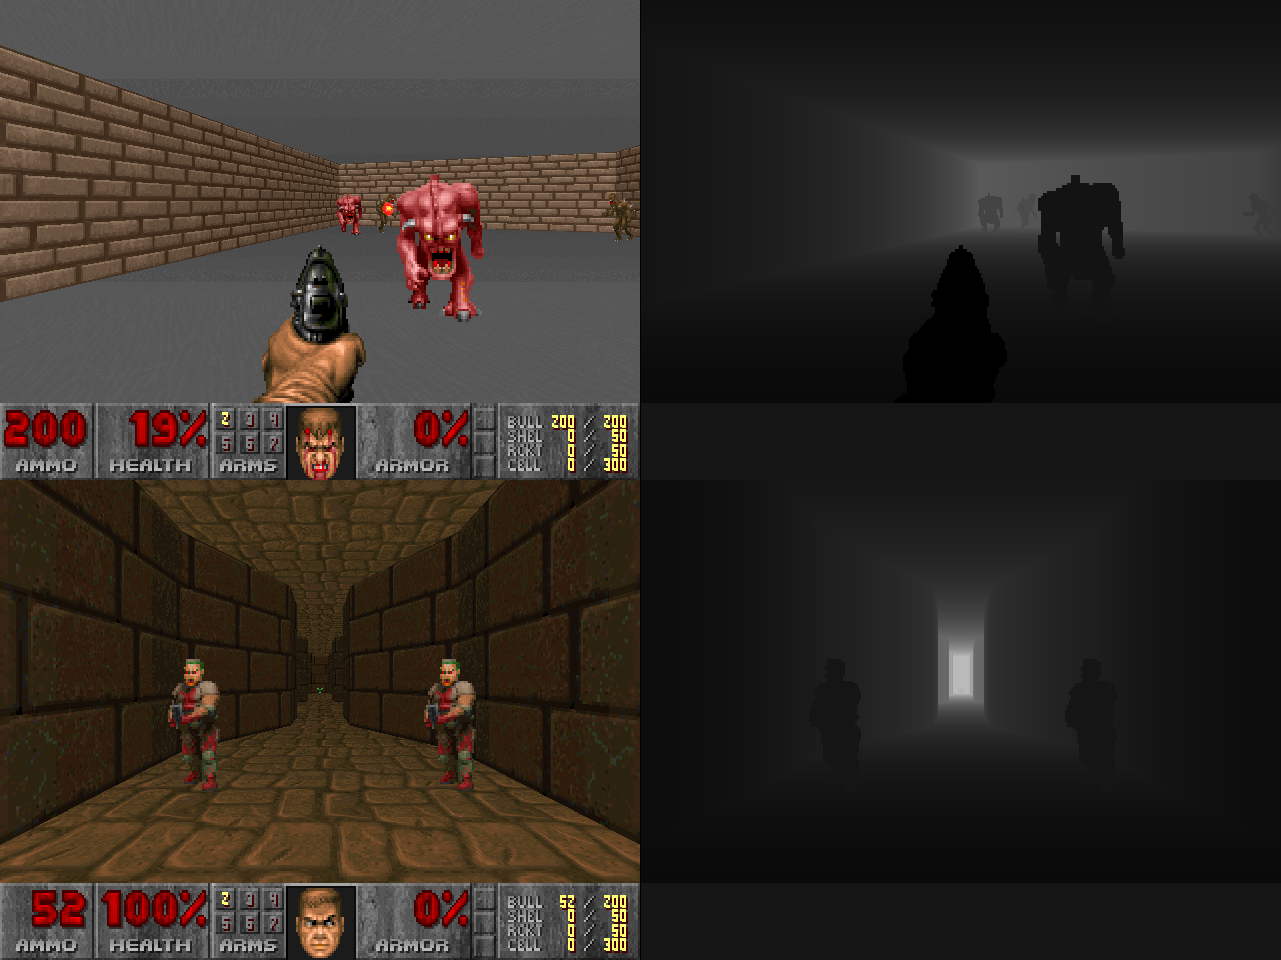
\includegraphics[scale=0.3]{zbuffer.png}
\caption{Example of implemented Zbuffer}
\label{fig:zbuffer}
\end{figure}

\subsubsection{Why multiplayer will not work in synchronous modes?}

Doom engine uses a peer-to-peer communication in multiplayer and requires tight synchronization between all game clients based on real time.
In synchronous modes time when next tic will be processed is unknown - too slow or too fast processing leads to desynchronization, unpredictable game behaviors and errors in processing. Therefore, the game network code has been disabled in synchronous modes.

\subsubsection{Why OSX is not supported?}

All Vizia environment code is OSX compatible. Due to the lack of access to OSX machine developers have not tested build system for it.

\subsubsection{Why game and scenario files are separated?}

Doom engine uses diffrent type of files for storing data and resources. (WAD and PK3 files) It allows to load main game resources from one file and many additional (scenario) resources from separate files. 

\section{Performance}
Table with some fps ratings and a graph.
Conclusions: it's fast enough, any reasonably good AI will be much slower during learning process.



